\chapter{\textbf{Конструкторский раздел}}

Задача этого проекта -- удостовериться, что пользователь отправляет валидный документ и дать ответ, какой тип документа он загрузил. 

Классификатор получает входные данные: фотографию документа. На выходе классификатор сообщает, что он получил (паспорт, водительское удостоверение и так далее) и насколько он уверен в правильности ответа.

\section{Функциональная модель}

На рисунке \ref{img:idef0} изображена функциональная модель, отображающая структуру и функции программного обеспечения. 

\begin{figure}[H]
	\centering
	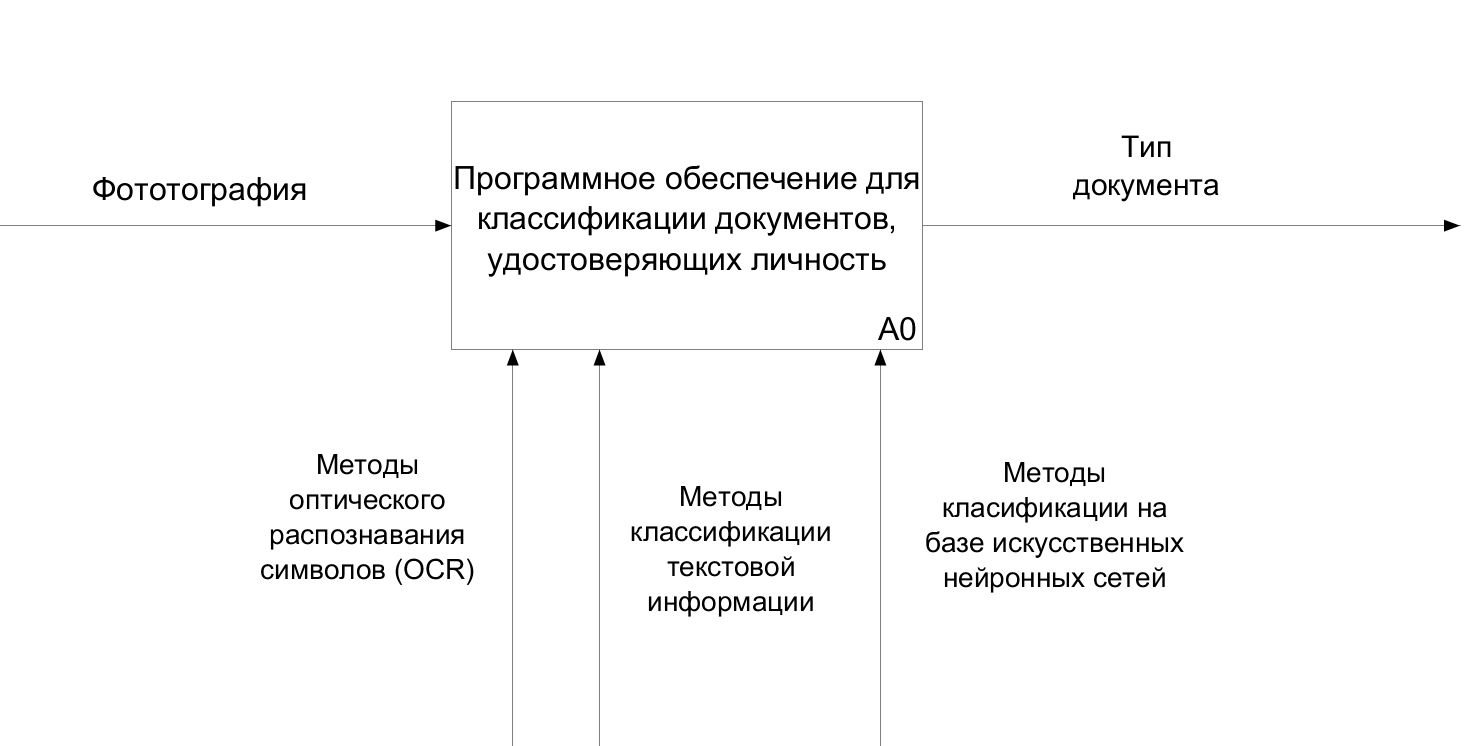
\includegraphics[scale=0.3]{idef0}
	\caption{Функциональная модель разрабатываемого ПО. }
	\label{img:idef0}
\end{figure}

На рисунке \ref{img:idef01} изображена функциональная модель первого уровня. 

\begin{figure}[H]
	\centering
	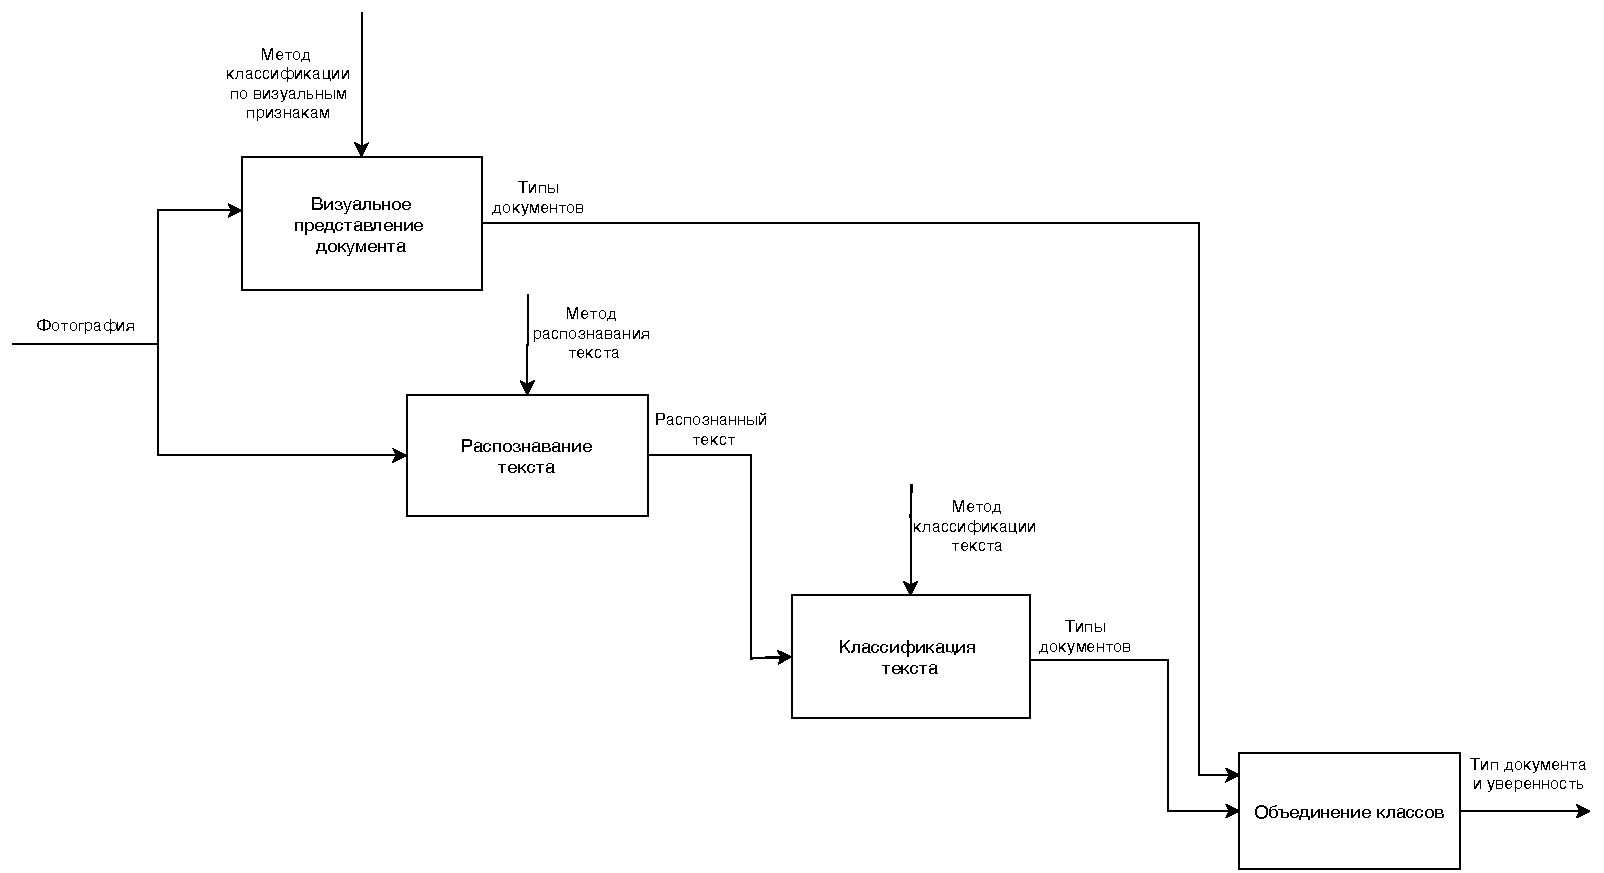
\includegraphics[scale=0.3]{idef01}
	\caption{Функциональная модель первого уровня. }
	\label{img:idef01}
\end{figure}
